\documentclass[11pt]{article}
\usepackage{../mymacros}

\setlength{\parindent}{0em}
\setlength{\parskip}{1em}

\begin{document}

% Set header and footer

\pagestyle{fancy}
\fancyhf{}
\rhead{PHYS 472}
\lhead{Assignment 2}
\cfoot{\thepage}

\begin{enumerate}[label=\textbf{\arabic*}.]
    \item % q1
    \begin{enumerate}
        \item % q1a
            We know that the expectation value of the square of the separation distance between the two particles is given by
            \begin{align*}
                \expval{(x_1 - x_2)^2} = \expval{x_1^2} + \expval{x_2^2} - 2\expval{x_1 x_2} \text{.} 
            \end{align*}
            In particular, for a system made of two distinguishable particles with $\Psi(x_1,x_2) = \psi_m(x_1)\psi_n(x_2)$, we have
            \begin{align*}
                \expval{(x_1 - x_2)^2}_\mathrm{disting.} = \expval{x^2}_m + \expval{x^2}_n - 2\expval{x}_m \expval{x}_n \text{;}
            \end{align*}
            on the other hand, for a system made of two identical particles with
            \begin{align*}
                \Psi(x_1,x_2) = \frac{1}{\sqrt{2}}\left[\psi_m(x_1)\psi_n(x_2) \pm \psi_n(x_1) \psi_m(x_2) \right] \text{,}
            \end{align*}
            we have
            \begin{align*}
                \expval{(x_1 - x_2)^2}_{\pm} =\expval{(x_1 - x_2)^2}_\mathrm{disting.} \mp 2\left| \expval{x}_{mn} \right|^2 \text{,}
            \end{align*}
            where
            \begin{align*}
                \expval{x}_{mn} \equiv \bra{m}x\ket{n} \text{.}
            \end{align*}
            Now recall that with quantum harmonic oscillators, we can work with ladder operators. In particular, the position operator in terms of ladder operators is given by
            \begin{align*}
                x = \sqrt{\frac{\hbar}{2m_0 \omega}} \left(a + a^\dagger\right)
            \end{align*}
            so that
            \begin{align*}
                x^2 &= \frac{\hbar}{2m_0 \omega} \left(aa + a^\dagger a^\dagger + aa^\dagger + a^\dagger a\right) \\
                &= \frac{2}{\hbar\omega} \hat{H} \text{.}
            \end{align*}
            Lastly let us recall the fact that for harmonic oscillators, $\expval{x} = 0$.
            \begin{enumerate}[label=(\roman*)]
                \item Distinguishable particles:
                    \begin{align*}
                        \expval{(x_1 - x_2)^2}_\mathrm{disting.} &= \expval{x^2}_m + \expval{x^2}_n - \cancelto{0}{2\expval{x}_m \expval{x}_n} \\
                        &= \frac{\hbar}{2m_0\omega}\left\{ \bra{m}x^2 \ket{m} + \bra{n}x^2 \ket{n} \right\} \\
                        &= \frac{\hbar}{2m_0 \omega}\left\{ \bra{m}\left(aa^\dagger + a^\dagger a\right)\ket{m} + \bra{n}\left(aa^\dagger + a^\dagger a\right)\ket{n} \right\} \\
                        &= \frac{\hbar}{2m_0\omega}\frac{2}{\hbar\omega} \left\{\bra{m}\hat{H}\ket{m} + \bra{n}\hat{H}\ket{n}\right\} \\
                        &= \frac{\hbar}{m_0 \omega^2} \left( E_m + E_n \right) \\
                        &= \frac{\hbar}{m_0 \omega^2} \hbar\omega \left(m + \frac{1}{2} + n + \frac{1}{2}\right) \\
                        &= \boxed{\frac{\hbar}{m_0\omega}(m + n + 1)  \text{.}}
                    \end{align*}

                \item Bosons:
                    \begin{align*}
                        \expval{x}_{mn} &= \bra{m}x\ket{n} \\
                        &= \sqrt{\frac{\hbar}{2m_0 \omega}} \bra{m} a^\dagger + a \ket{n} \\
                        &= \sqrt{\frac{\hbar}{2m_0 \omega}}\left\{ \bra{m}a^\dagger \ket{n} + \bra{m} a \ket{n} \right\} \\
                        &= \sqrt{\frac{\hbar}{2m_0 \omega}} \left\{\sqrt{n+1}\braket{m}{n+1} + \sqrt{n}\braket{m}{n-1}\right\} \\
                        &= \sqrt{\frac{\hbar}{2m_0 \omega}} \left( \delta_m^{n+1}\sqrt{n+1} + \delta_m^{n-1}\sqrt{n} \right) \text{.}
                    \end{align*}
                    Similarly, we found
                    \begin{align*}
                        \expval{x}_{nm} &= \sqrt{\frac{\hbar}{2m_0 \omega}} \left( \delta_m^{n+1}\sqrt{m} + \delta_m^{n-1}\sqrt{m+1} \right) \text{.}
                    \end{align*}
                    Therefore,
                    \begin{align*}
                        |\expval{x}_{mn}|^2 &= \expval{x}_{mn}\expval{x}_{nm} \\
                        &= \frac{\hbar}{2m_0 \omega}  \underbrace{\left(\delta_m^{n+1}\sqrt{m}\sqrt{n+1} + \delta_m^{n-1}\sqrt{m+1}\sqrt{n}\right)}_{>\, 0} \text{.}
                    \end{align*}
                    All in all,
                    \begin{align*}
                        \expval{(x_1 - x_2)^2}_\mathrm{bosons} &= \expval{(x_1 - x_2)^2}_\mathrm{disting.} - 2\left| \expval{x}_{mn} \right|^2 \\
                        &= \boxed{\frac{\hbar}{m_0\omega}\left(m+n+1 - \delta_m^{n+1}\sqrt{m}\sqrt{n+1} - \delta_m^{n-1}\sqrt{m+1}\sqrt{n} \right) \text{.}}
                    \end{align*}
                
                \item Fermions:
                    \newline
                    Analogously,
                    \begin{align*}
                        \expval{(x_1 - x_2)^2}_\mathrm{fermions} &= \expval{(x_1 - x_2)^2}_\mathrm{disting.} + 2\left| \expval{x}_{mn} \right|^2 \\
                        &= \boxed{\frac{\hbar}{m_0\omega}\left(m+n+1 + \delta_m^{n+1}\sqrt{m}\sqrt{n+1} + \delta_m^{n-1}\sqrt{m+1}\sqrt{n} \right) \text{.}}
                    \end{align*}
            \end{enumerate}

        \item % 1b
            With first two Hermite polynomials $H_0(\xi)=1$ and $H_1(\xi) = 2\xi$, we can write down
            \begin{align*}
                \psi_0(x) &= \left(\frac{m_0 \omega}{\pi\hbar}\right)^{1/4} H_0(\xi) e^{-\xi^2/2} = \left(\frac{m_0 \omega}{\pi\hbar}\right)^{1/4} e^{-\xi^2/2} \text{;} \\
                \psi_1(x) &= \frac{1}{\sqrt{2}} \left(\frac{m_0 \omega}{\pi\hbar}\right)^{1/4} H_1(\xi) e^{-\xi^2/2} = \frac{1}{\sqrt{2}} \left(\frac{m_0 \omega}{\pi\hbar}\right)^{1/4} \left(2\xi\right) e^{-\xi^2/2} \text{.}
            \end{align*}
            Then for distinguishable particless:
            \begin{align*}
                \Psi_\mathrm{disting.}(x_1,x_2) &= \psi_0(x_1) \psi_1(x_2) \\
                &= \boxed{\sqrt{2} \left(\frac{m_0 \omega}{\pi\hbar}\right)^{1/2} \xi_2 \exp\left(-\frac{\xi_1^2}{2} - \frac{\xi_2^2}{2}\right)}
            \end{align*}
            so that
            \begin{align*}
                \boxed{|\Psi_\mathrm{disting.}(x_1,x_2)|^2 = \frac{2}{\pi x_0^2} \xi_2^2 \exp(-\xi_1^2 - \xi_2^2) \text{.}}
            \end{align*}
            Now for identical particles:
            \begin{align*}
                \Psi_{\pm}(x_1,x_2) &= \frac{1}{\sqrt{2}} \left[\psi_0(x_1)\psi_1(x_2) \pm \psi_1(x_1)\psi_0(x_2)\right] \\
                &= \frac{1}{\sqrt{2}} \left(\Psi_\mathrm{disting.}(x_1,x_2) \pm \Psi_\mathrm{disting.}(x_2,x_1)\right) \\
                &= \boxed{\left(\frac{m_0 \omega}{\pi\hbar}\right)^{1/2} \exp\left(-\frac{\xi_1^2}{2} - \frac{\xi_2^2}{2}\right) (\xi_2 \pm \xi_1)}
            \end{align*}
            so that
            \begin{align*}
                \boxed{|\Psi_{\pm}(x_1,x_2)|^2 = \frac{1}{\pi x_0^2} \exp(-\xi_1^2 - \xi_2^2) (\xi_2 \pm \xi_1)^2 \text{.}}
            \end{align*}

            All in all,
            \begin{equation*}
                \boxed{
                    \begin{aligned}
                        \pi x_0^2 |\Psi(x_1, x_2)|^2 = \begin{cases}
                            2\xi_2^2 \exp(-\xi_1^2 - \xi_2^2) \qquad & \text{distinguishable,} \\
                            \exp(-\xi_1^2 - \xi_2^2) (\xi_2 + \xi_1)^2 & \text{bosons,} \\
                            \exp(-\xi_1^2 - \xi_2^2) (\xi_2 - \xi_1)^2 & \text{fermions.}
                        \end{cases}
                    \end{aligned}
                }
            \end{equation*}

            Now if $x_1 = x_2 = x$, then
            \begin{equation*}
                \boxed{
                    \begin{aligned}
                        \pi x_0^2 |\Psi(x, x)|^2 = \begin{cases}
                            2\xi^2 \exp(-2\xi^2) \qquad & \text{distinguishable,} \\
                            4\xi^2\exp(-2\xi^2) & \text{bosons,} \\
                            0 & \text{fermions.}
                        \end{cases}
                    \end{aligned}
                }
            \end{equation*}
    \end{enumerate}
\end{enumerate}

\begin{lstlisting}
    atSamePosition = Plot[{2 \[Xi]^2 Exp[-2 \[Xi]^2], 4 \[Xi]^2 Exp[-2 \[Xi]^2], 0}, {\[Xi],  -2, 2}, PlotLegends -> Placed[{"distinguishable", "bosons", "fermions"}, {0.89, 0.75}]]
\end{lstlisting}

\begin{figure}[H] % the [h!] argument attempts to place the figure here in the document
    \centering
    \resizebox{0.8\textwidth}{!}{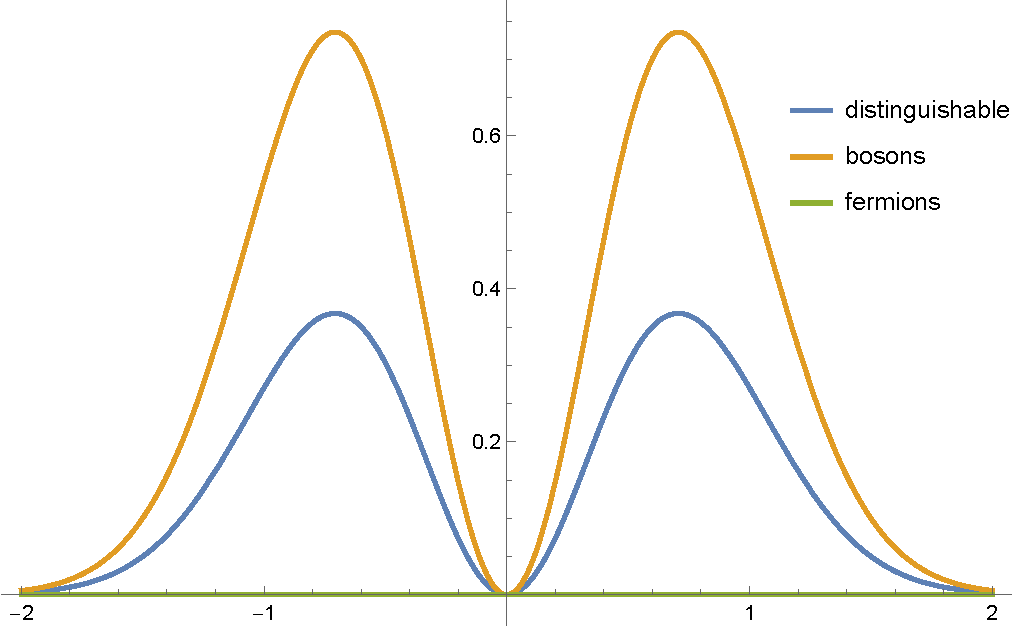
\includegraphics{atSamePosition.pdf}} % resizes the figure to 80% of the text width while maintaining the aspect ratio
    \caption{A two-particles system at $x_1 = x_2 = x$. By the Pauli exclusion principle, two fermions cannot be found at the same position. Due to exchange ``forces'' arising from symmetrization, two bosons are more likely to be close to each other.}
    \label{fig:fig1}
\end{figure}

% \begin{lstlisting}
%     plot1 = Plot3D[
%         4 xi2^2 Exp[-xi1^2/2 - xi2^2/2], {xi1, -3, 3}, {xi2, -3, 3}, 
%         AxesLabel -> {Subscript[\[Xi], 1], Subscript[\[Xi], 2], 
%         Superscript[Abs[Subscript[\[Psi], Row[{"(", Subscript[\[Xi], 1], ", ", Subscript[\[Xi], 2], ")"}]]], 2]}, PlotStyle -> Opacity[0.5], Mesh -> None, PlotRange -> All];

%     plot2 = Plot3D[
%         4 xi2^2 Exp[-xi1^2/2 - xi2^2/2] (xi1 + xi2)^2, {xi1, -3, 
%         3}, {xi2, -3, 3}, PlotStyle -> {Opacity[0.5], Red}, Mesh -> None, PlotRange -> All];

%     plot3 = Plot3D[
%         4 xi2^2 Exp[-xi1^2/2 - xi2^2/2] (xi1 - xi2)^2, {xi1, -3, 
%         3}, {xi2, -3, 3}, PlotStyle -> {Opacity[0.5], Blue}, Mesh -> None, PlotRange -> All];

%     atDifferentPosition = Show[
%         Legended[plot1, Placed[Style["distinguishable", FontColor -> Orange], {0.15, 0.8}]], 
%         Legended[plot2, Placed[Style["bosons", FontColor -> Red], {0.15, 0.8}]], 
%         Legended[plot3, Placed[Style["fermions", FontColor -> Blue], {0.15, 0.8}]],ViewPoint -> {2.7, -3.5, 2.5}]
% \end{lstlisting}

\begin{lstlisting}
    distinguishable = Plot3D[2xi2^2 Exp[-xi1^2- xi2^2], {xi1, -3, 3}, {xi2, -3, 3}, AxesLabel -> {Subscript[\[Xi], 1], Subscript[\[Xi], 2], Superscript[Abs[Subscript[\[Psi], Row[{"(", Subscript[\[Xi], 1], ", ", Subscript[\[Xi], 2], ")"}]]], 2]}, Mesh -> None, PlotRange -> All, ColorFunction -> Function[{x, y, z}, ColorData["Rainbow"][z]], ColorFunctionScaling -> True, Mesh -> None, ViewPoint -> {0, 0, Infinity}]
\end{lstlisting}

\begin{lstlisting}
    bosons = Plot3D[Exp[-xi1^2 - xi2^2] (xi1 + xi2)^2, {xi1, -3, 3}, {xi2, -3, 3}, AxesLabel -> {Subscript[\[Xi], 1], Subscript[\[Xi], 2], Superscript[Abs[Subscript[\[Psi], Row[{"(", Subscript[\[Xi], 1], ", ", Subscript[\[Xi], 2], ")"}]]], 2]}, Mesh -> None, PlotRange -> All, ColorFunction -> Function[{x, y, z}, ColorData["Rainbow"][z]], ColorFunctionScaling -> True, Mesh -> None, ViewPoint -> {0, 0, Infinity}]
\end{lstlisting}

\begin{lstlisting}
    fermions = Plot3D[Exp[-xi1^2 - xi2^2] (xi1 - xi2)^2, {xi1, -3, 3}, {xi2, -3, 3}, AxesLabel -> {Subscript[\[Xi], 1], Subscript[\[Xi], 2], Superscript[Abs[Subscript[\[Psi], Row[{"(", Subscript[\[Xi], 1], ", ", Subscript[\[Xi], 2], ")"}]]], 2]}, Mesh -> None, PlotRange -> All, ColorFunction -> Function[{x, y, z}, ColorData["Rainbow"][z]], ColorFunctionScaling -> True, Mesh -> None, ViewPoint -> {0, 0, Infinity}]
\end{lstlisting}

\begin{figure}[h!]
    \centering
    \subfloat[Distinguishable particles]{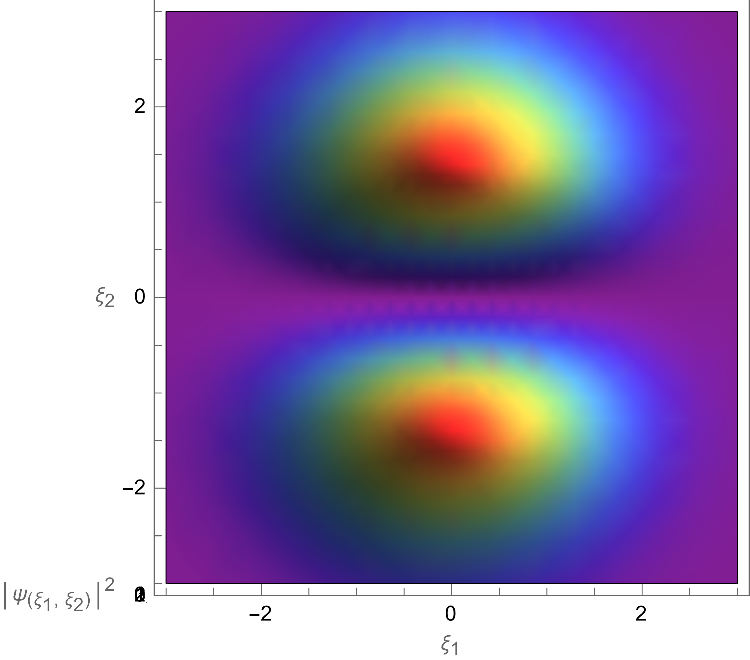
\includegraphics[width=0.3\textwidth]{atDifferentPositions_distinguishable_3d.pdf}}
    \hfill
    \subfloat[Bosons]{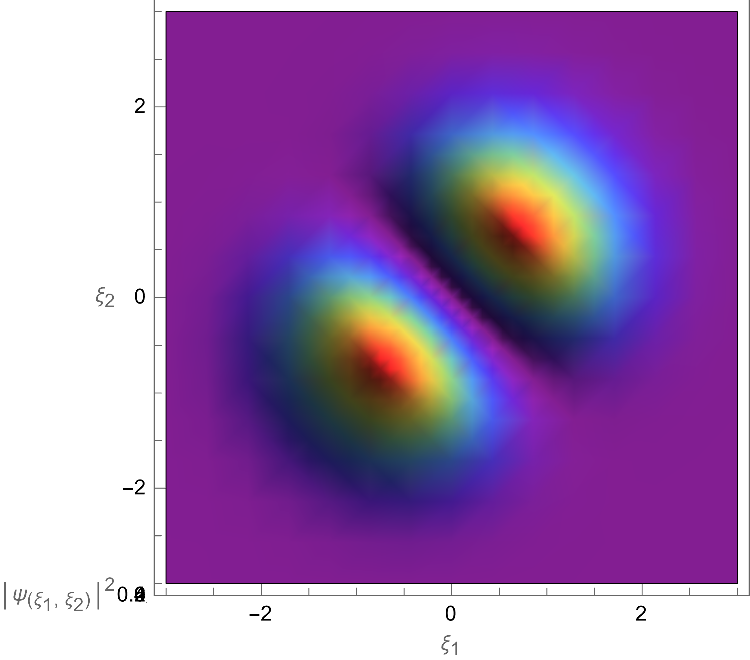
\includegraphics[width=0.3\textwidth]{atDifferentPositions_bosons_3d.pdf}}
    \hfill
    \subfloat[Fermions]{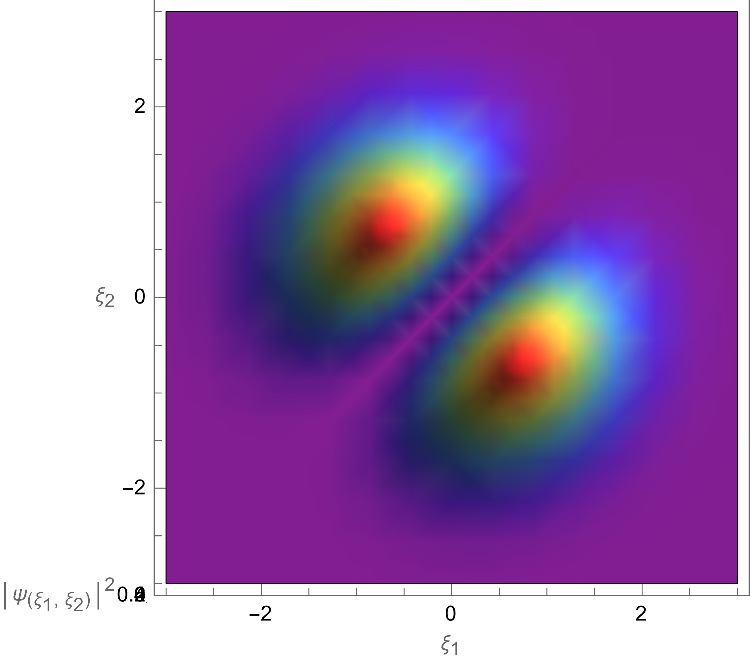
\includegraphics[width=0.3\textwidth]{atDifferentPositions_fermions_3d.pdf}}
    \caption{Top view of $\pi x_0^2 |\Psi(x_1,x_2)|^2 \text{ vs. } \xi_1 \text{ and } \xi_2$. Note that looking at the section of the $\xi_1 = \xi_2$ plane in this 3d plot, we obtain the result of Figure \ref{fig:fig1}.}
    \label{fig:fig2}
\end{figure}


    



\end{document}